\documentclass[11pt]{article}
\usepackage[T1]{fontenc}
\usepackage{amsmath,amssymb,amsthm,mathtools,mathrsfs}
\usepackage{graphicx}
\usepackage{geometry}
\usepackage[colorlinks=true,linkcolor=blue,citecolor=blue,urlcolor=blue]{hyperref}
\geometry{margin=1in}

\newtheorem{theorem}{Theorem}
\newtheorem{lemma}{Lemma}
\newcommand{\R}{\mathbb R}
\newcommand{\Sph}{\mathbb S}
\newcommand{\E}{\mathscr E}
\newcommand{\cK}{\mathcal K}
\newcommand{\norm}[1]{\left\lVert #1\right\rVert}
\newcommand{\abs}[1]{\left\lvert #1\right\rvert}

\title{The integer-\(L^1\) endpoints in higher-order affine Sobolev inequalities}
\author{Run fa\_banach\_001, agent lane 14}
\date{2026-08-11}

\begin{document}
\maketitle

\begin{abstract}
Bullion--Gauthier's Theorems 1.1 and 1.2 leave open the cases in which the
upper smoothness is an integer \(m\geq2\) and the upper exponent is \(1\).
We close both omissions.  The affine energy is the reciprocal-volume scale of
the star body
\[
 \cK_f=\{v\in\R^N:\norm{\partial_v^m f}_{L^1}\leq1\}.
\]
A maximal-determinant tuple in this body yields a unimodular basis whose total
pure-derivative cost is \(O(\E_{m,1}(f))\).  In those coordinates the pure
power operator is elliptic and canceling, so Van Schaftingen's limiting
Sobolev estimates give exactly the missing lower norms.  No mixed-derivative
estimate is used, and Ornstein's non-inequality is bypassed.
\end{abstract}

\section{Source statements and omitted cases}

Let \(N\geq2\).  For an integer \(m\geq1\), the source \cite{BG} defines
\[
 a_f(v):=\norm{\partial_v^m f}_{L^1(\R^N)},\qquad
 \E_{m,1}(f)
 =\sigma_N^{(N+m)/N}
 \left(\int_{\Sph^{N-1}}a_f(\theta)^{-N/m}\,d\mathcal H^{N-1}(\theta)
 \right)^{-m/N},
\]
where \(\sigma_N=\mathcal H^{N-1}(\Sph^{N-1})\).

Theorem 1.1 of \cite{BG} states the strong critical affine Sobolev inequality
possibly except when \(s\geq2\) is an integer and \(p=1\).  The definition and
exception occur on source PDF page 2.

\begin{figure}[ht]
\centering
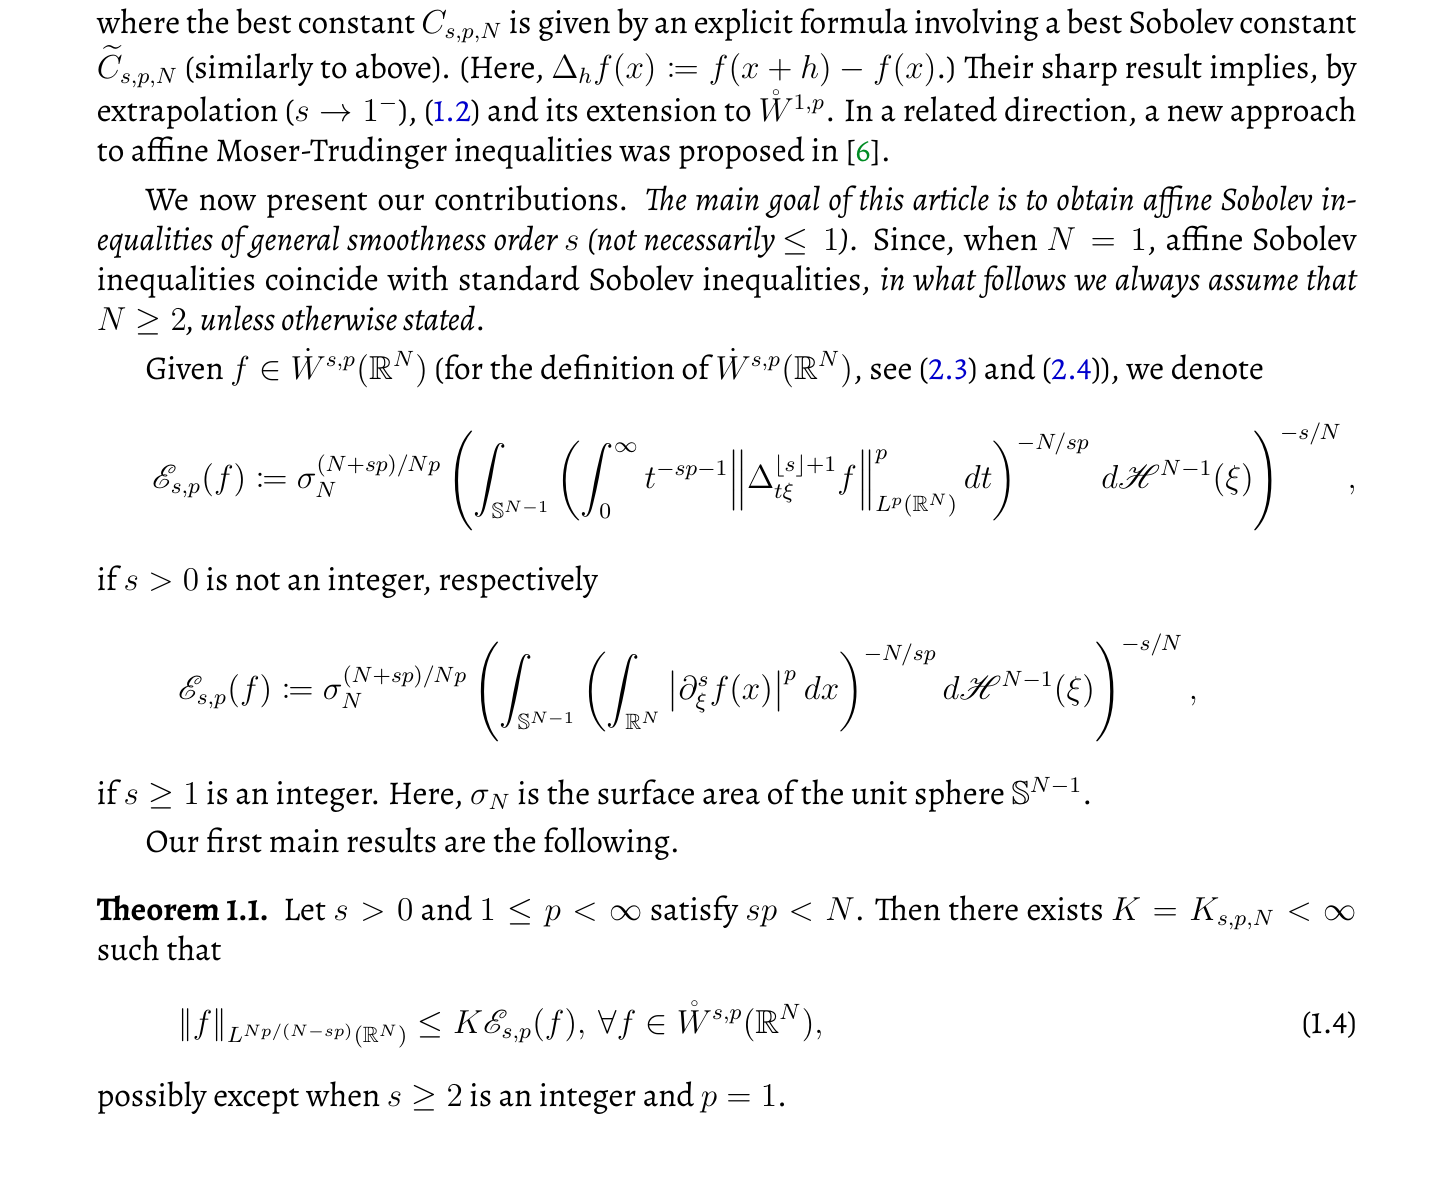
\includegraphics[width=0.98\linewidth]{figures/source_definition_theorem11-02.png}
\caption{The integer affine energy and the omitted case in Theorem 1.1 of
\cite{BG}, source PDF page 2.}
\end{figure}

Theorem 1.2 compares two affine energies on the Sobolev line
\(s_2-N/p_2=s_1-N/p_1\), again possibly except when the upper pair is an
integer \(s_2\geq2\) and \(p_2=1\).  This appears on source PDF page 3.

\begin{figure}[ht]
\centering
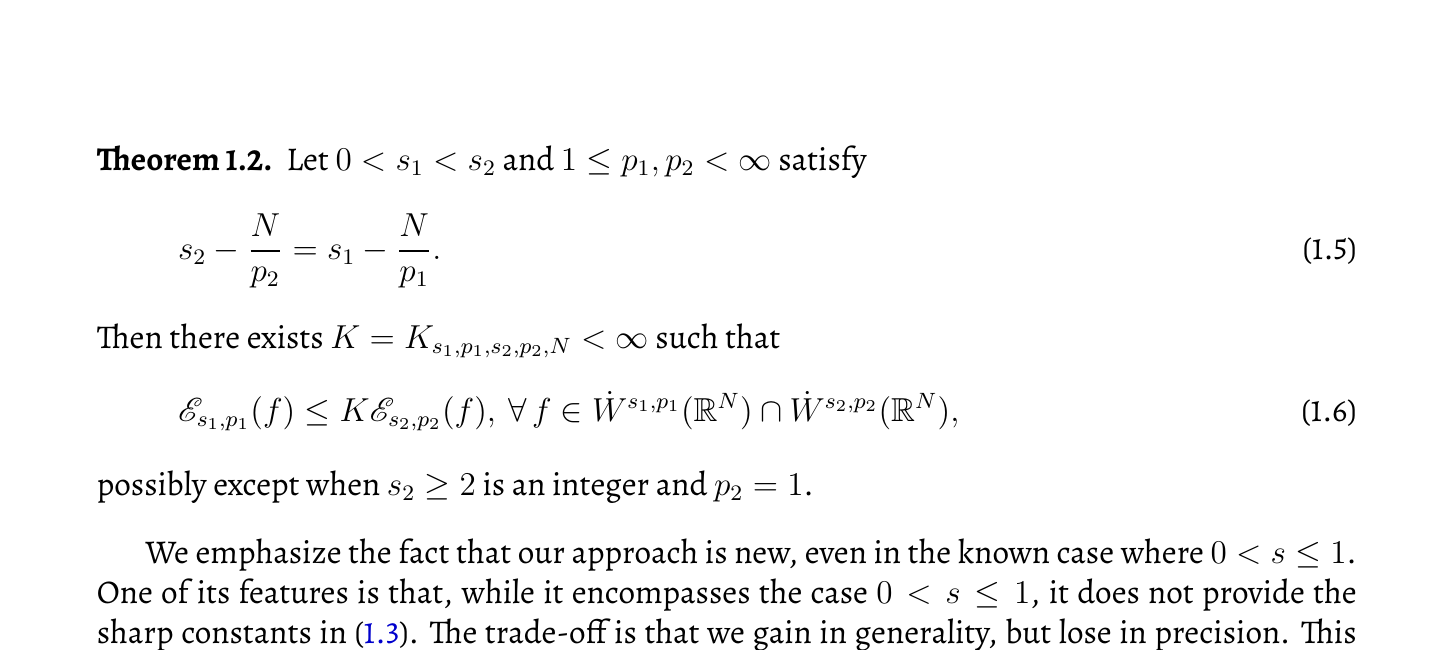
\includegraphics[width=0.98\linewidth]{figures/source_theorem12-03.png}
\caption{The omitted case in Theorem 1.2 of \cite{BG}, source PDF page 3.}
\end{figure}

Thus the two extracted questions are whether, for every integer \(m\geq2\),
\[
 \norm{f}_{L^{N/(N-m)}}\lesssim\E_{m,1}(f)\quad(m<N),
\]
and, more generally, whether
\[
 \E_{s,p}(f)\lesssim\E_{m,1}(f)
 \quad\text{when}\quad 0<s<m,\qquad m-N=s-\frac Np.
\]

\section{Proof intuition}

The source route tries to control a full order-\(m\) Sobolev tensor after an
optimal unimodular coordinate change.  At \(p=1\), mixed derivatives make this
incompatible with Ornstein's non-inequality.  The desired conclusions need
only \(N\) pure derivatives.  For a fixed basis these form an elliptic,
canceling system, and limiting Sobolev theory controls the critical lower norm
directly.

It remains to choose the basis.  The function
\(a_f(v)=\norm{\partial_v^m f}_1\) is \(m\)-homogeneous, so its unit sublevel
set is a symmetric star body.  Its radial volume is exactly the negative
spherical mean defining \(\E_{m,1}\).  A maximal-determinant argument,
requiring no convexity, extracts a unimodular basis with total cost
\(O(\E_{m,1})\).  The geometry and the canceling estimate have precisely the
same critical scaling.

\section{The two ingredients}

\begin{lemma}[Maximal-determinant selection]\label{lem:selection}
Suppose \(a_f\) is continuous and positive on \(\Sph^{N-1}\).  There is a
basis \(v_1,\ldots,v_N\) with \(\det(v_1,\ldots,v_N)=1\) and
\[
 \sum_{i=1}^N a_f(v_i)\leq C_{N,m}\E_{m,1}(f).
\]
\end{lemma}

\begin{proof}
Set \(\cK_f=\{v:a_f(v)\leq1\}\).  It is a compact symmetric star body with
nonempty interior, and polar coordinates give
\begin{equation}\label{eq:volume}
 \abs{\cK_f}
 =\frac1N\int_{\Sph^{N-1}}a_f(\theta)^{-N/m}\,d\mathcal H^{N-1}(\theta),
\qquad
 \abs{\cK_f}^{-m/N}
 =N^{m/N}\sigma_N^{-(N+m)/N}\E_{m,1}(f).
\end{equation}
Choose \(w_1,\ldots,w_N\in\cK_f\) maximizing
\(d=\abs{\det(w_1,\ldots,w_N)}>0\).  If
\(x=\sum_i\alpha_iw_i\in\cK_f\), replacing column \(i\) by \(x\) gives
\(\abs{\alpha_i}d\leq d\); hence \(\abs{\alpha_i}\leq1\).  Therefore
\[
 \cK_f\subseteq
 \left\{\sum_i\alpha_iw_i:\abs{\alpha_i}\leq1\right\},
\qquad \abs{\cK_f}\leq2^N d.
\]
After changing one sign, set \(v_i=d^{-1/N}w_i\).  The determinant is one and
\[
 \sum_i a_f(v_i)
 =d^{-m/N}\sum_i a_f(w_i)
 \leq N d^{-m/N}
 \leq N2^m\abs{\cK_f}^{-m/N}.
\]
Now use \eqref{eq:volume}.
\end{proof}

\begin{lemma}[Pure powers form a canceling system]\label{lem:canceling}
For \(g\in C_c^\infty(\R^N)\):
\begin{enumerate}
\item if \(m<N\), then
\[
 \norm{g}_{L^{N/(N-m)}}\leq C_{N,m}
 \sum_{i=1}^N\norm{\partial_i^m g}_{L^1};
\]
\item if \(0<s<m\), \(1<p<\infty\), and
\(1/p-s/N=1-m/N\), then
\[
 \abs{g}_{\dot W^{s,p}}\leq C_{N,m,s,p}
 \sum_{i=1}^N\norm{\partial_i^m g}_{L^1},
\]
with the integer Sobolev seminorm when \(s\) is integral and the
Sobolev--Slobodeckij seminorm of \cite{BG} otherwise.
\end{enumerate}
\end{lemma}

\begin{proof}
For \(A(D)g=(\partial_1^m g,\ldots,\partial_N^m g)\), the scalar symbol is
\[
 A(\xi)t=t(\xi_1^m,\ldots,\xi_N^m).
\]
It is elliptic.  It is also canceling in the sense of \cite{VS}, since
\[
 \bigcap_{\xi\neq0}A(\xi)[\R]
 \subseteq\bigcap_{j=1}^N A(e_j)[\R]
 =\bigcap_{j=1}^N\operatorname{span}\{e_j\}=\{0\},
\]
using \(N\geq2\).  Van Schaftingen's Theorem 1.3 \cite{VS} gives
\[
 \norm{D^{m-1}g}_{L^{N/(N-1)}}
 \leq C\sum_i\norm{\partial_i^m g}_{L^1}.
\]
The classical homogeneous Sobolev embedding of order \(m-1\) gives part 1.
For part 2, use Proposition 8.12 of \cite{VS} with
\(\dot F^s_{p,2}=\dot W^{s,p}\) when \(s\) is integral, and Proposition 8.13
with \(\dot B^s_{p,p}=\dot W^{s,p}\) when \(s\) is nonintegral.  Their
parameter identity is exactly \(1/p-s/N=1-m/N\).
\end{proof}

\section{Full endpoint theorem}

\begin{theorem}\label{thm:main}
Let \(N\geq2\) and let \(m\geq2\) be an integer.
\begin{enumerate}
\item If \(m<N\), then
\[
 \norm{f}_{L^{N/(N-m)}(\R^N)}
 \leq C_{N,m}\E_{m,1}(f),
 \qquad f\in\mathring W^{m,1}(\R^N).
\]
\item If \(0<s<m\), \(1\leq p<\infty\), and
\(m-N=s-N/p\), then
\[
 \E_{s,p}(f)\leq C_{N,m,s,p}\E_{m,1}(f),
 \qquad
 f\in\dot W^{s,p}(\R^N)\cap\dot W^{m,1}(\R^N).
\]
\end{enumerate}
Consequently the omitted integer-\(L^1\) cases in both Theorems 1.1 and 1.2
of \cite{BG} hold.
\end{theorem}

\begin{proof}
First let \(f\in C_c^\infty(\R^N)\), \(f\neq0\).  Then \(a_f\) is continuous
and positive on the sphere: if \(a_f(v)=0\), the restriction of \(f\) to
almost every line parallel to \(v\) is a polynomial of degree at most
\(m-1\), and compact support forces it to vanish.  Lemma
\ref{lem:selection} supplies \(v_1,\ldots,v_N\) such that
\begin{equation}\label{eq:cost}
 \det(v_1,\ldots,v_N)=1,\qquad
 \sum_i\norm{\partial_{v_i}^m f}_{L^1}
 \leq C_{N,m}\E_{m,1}(f).
\end{equation}
Let \(T\in\mathrm{SL}_N\) have columns \(v_i\), and set \(g=f\circ T\).
Then
\[
 \norm{\partial_i^m g}_{L^1}
 =\norm{\partial_{v_i}^m f}_{L^1}.
\]
If \(m<N\), Lemma \ref{lem:canceling} and \eqref{eq:cost} yield
\(\norm{g}_{L^{N/(N-m)}}\leq C\E_{m,1}(f)\).  The Lebesgue norm is unchanged
because \(\det T=1\), proving part 1.

For part 2, the parameter relation and \(s<m\) imply \(p>1\) and
\(s\in(m-N,m)\).  Lemma \ref{lem:canceling} gives
\[
 \abs{g}_{\dot W^{s,p}}
 \leq C\sum_i\norm{\partial_{v_i}^m f}_{L^1}
 \leq C\E_{m,1}(f).
\]
The source's Jensen estimate gives
\(\E_{s,p}(g)\leq C\abs{g}_{\dot W^{s,p}}\), while its affine-invariance
proposition gives \(\E_{s,p}(g)=\E_{s,p}(f)\).  Hence
\[
 \E_{s,p}(f)=\E_{s,p}(g)
 \leq C\abs{g}_{\dot W^{s,p}}
 \leq C\E_{m,1}(f).
\]
Crucially, the ordinary seminorm is used only for \(g\); it is the affine
energy, not that seminorm, which is transported back through \(T\).

For the source spaces, Appendix A of \cite{BG} gives
\(f_j\in C_c^\infty\) with
\(\abs{f_j-f}_{\dot W^{m,1}}\to0\).  The standard homogeneous embedding in
Appendix B gives convergence in the lower space (and in
\(L^{N/(N-m)}\) for part 1).  Moreover,
\[
 \sup_{\theta\in\Sph^{N-1}}
 \abs{a_{f_j}(\theta)-a_f(\theta)}
 \leq C_{N,m}\abs{f_j-f}_{\dot W^{m,1}}\longrightarrow0.
\]
The no-constant-direction lemma of \cite{BG} shows that \(a_f\) is positive
on the sphere whenever the relevant lower seminorm is nonzero: otherwise
\(\partial_v^m f=0\) would make every \(m\)-th finite difference along \(v\)
zero.  Compactness gives a positive minimum, so \(\E_{m,1}\) is continuous
under the displayed uniform convergence.  Passing to the limit proves the
claims.  If the lower seminorm in part 2 is zero, then
\(\E_{s,p}(f)=0\) and the conclusion is immediate.
\end{proof}

\section{Verification, scope, and novelty}

The determinant normalization is exact, and the selection lemma does not
assume convexity.  Cancellation is checked from the symbol rather than
inferred from ellipticity.  In the cross-order case \(p>1\) is automatic, so
the cited Triebel--Lizorkin/Besov estimates cover every parameter.  The only
coordinate-dependent norm is evaluated after the chosen change of variables;
the final left side is \(SL_N\)-invariant.  Thus no uniform control of mixed
derivatives is hidden in the argument.

This result closes Theorems 1.1 and 1.2 only.  It does not claim the omitted
integer-\(L^1\) minimizing-orbit coercivity in Theorem 1.4 or the reverse
comparisons involving the full order-\(m\) tensor.  Ornstein's obstruction
remains relevant there.

The four cheap run indexes were searched for arXiv:2506.10473, its exact
title, the integer-\(p=1\) endpoint, pure directional derivatives, canceling
operators, and the maximal-determinant star-body mechanism.  No duplicate was
found.  Bounded external searches on 2026-08-11 used the exact exception
phrases and the same combinations.  They found the current published source,
which still contains both exceptions, and the general canceling-operator
literature represented by \cite{VS}, but no paper closing these affine
endpoints.

The recommended verdict is \emph{candidate full solution, likely valid,
pending expert review}.  The highest-value checks are the identification of
the source seminorms with the spaces in Propositions 8.12--8.13, the
homogeneous density passage, and the no-constant-direction step for general
representatives.

\begin{thebibliography}{9}
\bibitem{BG}
Tristan Bullion--Gauthier,
\emph{Higher-order affine Sobolev inequalities},
Journal of Functional Analysis \textbf{290} (2026), no.~11, 111419;
arXiv:2506.10473v2.
\url{https://arxiv.org/abs/2506.10473}

\bibitem{VS}
Jean Van Schaftingen,
\emph{Limiting Sobolev inequalities for vector fields and canceling linear
differential operators},
Journal of the European Mathematical Society \textbf{15} (2013), 877--921;
arXiv:1104.0192.
\url{https://arxiv.org/abs/1104.0192}
\end{thebibliography}

\end{document}
